\documentclass[dvipdfmx]{jarticle}
\pagestyle{empty}
\usepackage{tikz}
\usetikzlibrary{calc,shapes}
\begin{document}
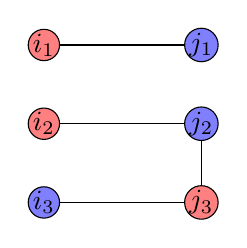
\begin{tikzpicture}
\node[draw,circle,inner sep=0pt,fill=red!50] (I1) at (0,0) {$i_1$};
\node[draw,circle,inner sep=0pt,fill=blue!50] (J1) at (2,0) {$j_1$};
\node[draw,circle,inner sep=0pt,fill=red!50] (I2) at (0,-1) {$i_2$};
\node[draw,circle,inner sep=0pt,fill=blue!50] (J2) at (2,-1) {$j_2$};
\node[draw,circle,inner sep=0pt,fill=blue!50] (I3) at (0,-2) {$i_3$};
\node[draw,circle,inner sep=0pt,fill=red!50] (J3) at (2,-2) {$j_3$};
\path[-] (I1) edge (J1) (I2) edge (J2) (I3) edge (J3);
\path[-] (J2) edge (J3);
\end{tikzpicture}
\end{document}